\documentclass{article}

\usepackage{graphicx}
\usepackage{float}

\usepackage{hyperref}

\usepackage[utf8]{inputenc}
\usepackage[francais]{babel}
\usepackage[T1]{fontenc}

\author{
    Yassir Karroum\\
    \texttt{ukarroum17@gmail.com}
    \and
    Reda Drissi\\
    \texttt{reda.drissi@yahoo.fr}
    \and
    Abdellah Elouassif\\
    \texttt{elouassif.28@gmail.com}
    \and
    Ikram Achlikhi\\
    \texttt{ash.ikram17@gmail.com}
    \and
    Nassima Barakat\\
    \texttt{nassima.bkt@gmail.com}
    \and
    Soukaina abelhad\\
    \texttt{abelhad.soukaina@gmail.com}
}

\title{Cahier de charges : \texttt{Jeu d'échecs}}
\begin{document}

\maketitle

\newpage

\tableofcontents

\newpage

\section{Présentation du jeu}

\subsection{Présentation en bref}

Le \texttt{jeu d’échecs} oppose deux joueurs de part et d’autre d’un plateau ou tablier appelé \texttt{échiquier} composé de soixante-quatre cases claires et sombres nommées les cases blanches et les cases noires. Les joueurs jouent à tour de rôle en déplaçant l'une de leurs seize pièces (ou deux pièces en cas de roque), claires pour le camp des blancs, sombres pour le camp des noirs. Chaque joueur possède au départ un \texttt{roi}, une \texttt{dame}, deux \texttt{tours}, deux \texttt{fous}, deux \texttt{cavaliers} et huit \texttt{pions}. Le but du jeu est d'infliger à son adversaire un échec et mat, une situation dans laquelle le roi d'un joueur est en prise sans qu'il soit possible d'y remédier \cite{wikiEchecs}.

\subsection{Régles du jeu}

Cette section représente les régles du jeu qu'on a jugé les plus importantes, cette liste n'est pas exaustive, pour pouvoir lire la totalité du réglement nous vous invitons à visiter le site du \texttt{FIDE} (Fédération internationale des echecs) \cite{fide}.

Ces articles ainsi que les images associés ont été copiés depuis le livret des régles d'échecs de la FIDE \cite{livreFide}.

Remarque : Nous avons délibérément omis l'Article 4 car nous n'avons pas jugé important de l'aborder ici .


\subsubsection{Article 1: Nature et objectifs du jeu d’échecs}

\begin{enumerate}


\item Le jeu d’échecs se joue entre deux adversaires  qui  déplacent  alternativement  des  pièces  sur  un  plateau carré appelé \texttt{échiquier}. Le joueur ayant les pièces blanches commence la partie. On dit qu’un joueur \texttt{a le trait} lorsque le coup de son adversaire a été \texttt{joué} .

\item L’objectif  de chaque  joueur  est  de  placer  le  roi  adverse \texttt{sous  une  attaque} de  telle  manière  que l’adversaire n’ait aucun coup légal. On dit que le joueur qui atteint ce but a \texttt{maté} le roi adverse et gagné la partie. Laisser son roi sous une attaque, exposer son roi à une attaque et aussi \texttt{prendre} le roi adverse n'est pas autorisé. L’adversaire dont le roi a été maté a perdu la partie.

\item Si la position est telle qu’aucun des deux joueurs n’a la possibilité de mater, la partie est nulle. \\

\end{enumerate}

\subsubsection{Article 2: La position initiale des pièces sur l’échiquier}

\begin{enumerate}

\item L’échiquier se compose d’une grille 8x8 de 64 cases identiques alternativement claires (les cases \texttt{blanches}) et foncées (les cases \texttt{noires}).
L’échiquier est placé entre les joueurs de telle manière que la case d’angle à la droite de chaque joueur
soit blanche.

\item Au début d’une partie, un joueur dispose de 16 pièces claires (les pièces \texttt{blanches}) et l’autre de 16 pièces foncées (les pièces \texttt{noires}).

\item La position initiale des pièces sur l'échiquier est la suivante :

\begin{figure}[H]
  \centering
  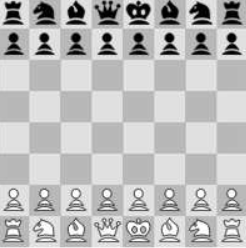
\includegraphics[scale=0.5]{init_pos.png}
  \caption{Position initiale des pièces}
\end{figure}

\item Les  huit  lignes  de  cases  verticales  sont  appelées \texttt{colonnes}.  Les  huit  lignes  de  cases  horizontales  sont appelées \texttt{rangées}. Une ligne droite de cases de même couleur, menant d’un bord de l’échiquier à un bord adjacent, est appelée \texttt{diagonale}.

\end{enumerate}

\subsubsection{Article 3: Mouvement des pièces}

\begin{enumerate}

\item Il n’est pas permis de déplacer une pièce sur une case occupée par une pièce de même couleur. Si une pièce se déplace sur une case occupée par une pièce adverse, cette dernière est prise et retirée de l’échiquier comme partie intégrante du coup. On dit qu’une pièce attaque une pièce adverse si elle peut éventuellement effectuer une prise sur cette case en accord avec les articles 3.2 à 3.8. Une pièce est considérée comme attaquant une case, même si cette pièce ne peut pas se déplacer sur cette case car elle mettrait ou laisserait son propre roi sous une attaque.

\item Le fou se déplace sur toute case d’une diagonale sur laquelle il se trouve.


\begin{figure}[H]
  \centering
  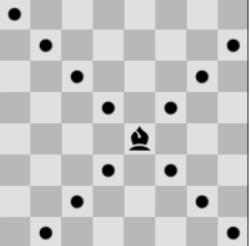
\includegraphics[scale=0.5]{fou.png}
  \caption{Mouvement du fou}
\end{figure}

\item La tour se déplace sur toute case de la colonne ou de la rangée sur laquelle elle se trouve.

\begin{figure}[H]
  \centering
  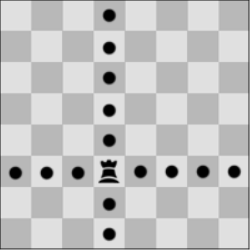
\includegraphics[scale=0.5]{tour.png}
  \caption{Mouvement de la tour}
\end{figure}

\item La dame se déplace sur toute case de la colonne, de la rangée ou d’une diagonale sur laquelle elle se trouve.

\begin{figure}[H]
  \centering
  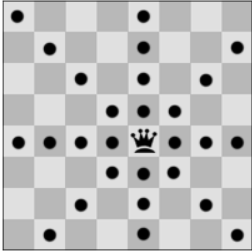
\includegraphics[scale=0.5]{reine.png}
  \caption{Mouvement de la dame}
\end{figure}

\item En effectuant ces mouvements, le fou, la tour ou la dame ne peuvent se déplacer au dessus d’aucune autre pièce.

\item Le cavalier se déplace sur l’une des cases les plus proches de celle sur laquelle il se trouve, mais pas sur la même colonne, rangée ou diagonale.

\begin{figure}[H]
  \centering
  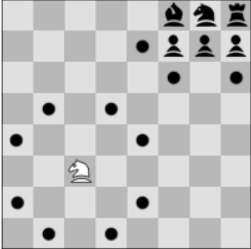
\includegraphics[scale=0.5]{cheval.png}
  \caption{Position initiale des pièces}
\end{figure}

\item 
    \begin{enumerate}
        \item Le pion se déplace sur la case inoccupée immédiatement devant lui sur la même colonne, ou
        \item à son premier coup, il peut se déplacer comme indiqué sur la figure suivante ou bien avancer de deux cases sur la même
        colonne à condition qu’elles soient toutes deux inoccupées, ou
        \item il se déplace sur une case occupée par une pièce adverse, située devant lui en diagonale sur une
        colonne adjacente, et capture ainsi cette pièce.

    \begin{figure}[H]
        \centering
        
\includegraphics[scale=0.5]{pion.png}
        \caption{Mouvement du pion}
    \end{figure}
        
        \item Un pion attaquant une case traversée par un pion adverse qui a avancé, d’un seul coup, de deux cases à partir de sa case initiale peut prendre ce pion comme si ce dernier n’avait avancé que d’une case.  Cette  prise n’est  légale qu’en  réponse  immédiate  à  cette  avancée  de  deux  cases  du  pion adverse. On l’appelle: \texttt{prise en passant}.
    \begin{figure}[H]
        \centering
        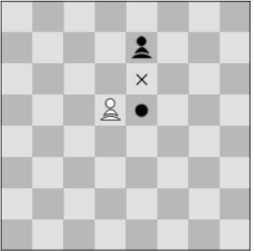
\includegraphics[scale=0.5]{passant.png}
        \caption{Prise en passant}
    \end{figure}
        \item Quand  un  pion  accède  à  la  rangée  la  plus  éloignée  de  sa  position  de  départ,  il  doit  être  échangé, comme partie intégrante du coup sur la même case, contre une nouvelle dame, tour, fou ou cavalier de la couleur du pion. Le joueur ne doit pas limiter son choix aux pièces qui ont été précédemment capturées. Cet échange d’un pion contre une autre pièce est appelé \texttt{promotion} et la pièce promue est immédiatement opérationnelle.
    \end{enumerate}

\item
    \begin{enumerate}
    \item Il y a deux façons différentes de déplacer le roi, soit : par un mouvement sur l’une des cases adjacentes qui n’est pas attaquée par une ou plusieurs pièces adverses

    \begin{figure}[H]
        \centering
        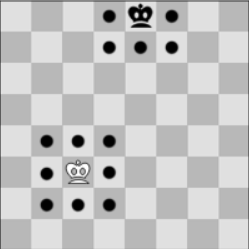
\includegraphics[scale=0.5]{roi.png}
        \caption{Mouvement du roi}
    \end{figure}

    soit par le \texttt{roque}. C’est un mouvement du roi et de l’une ou l’autre des tours de la même couleur, sur la première rangée du joueur, comptant pour un seul coup du roi et effectué de la manière suivante: le roi est déplacé de deux cases à partir de sa case initiale en direction de la tour sur sa case initiale ; cette tour est ensuite déplacée sur la dernière case que le roi vient de traverser.
    \begin{figure}[H]
        \centering
        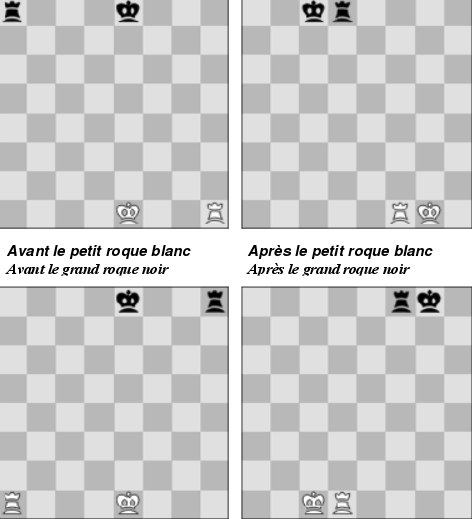
\includegraphics[scale=0.5]{roque.png}
        \caption{Mouvement du Le roque}
    \end{figure}

    \item 
        \begin{enumerate}
        \item Le droit de roquer est perdu :
            \begin{enumerate}
                \item si le roi a déjà bougé, ou
                \item avec une tour qui a déjà bougé.
            \end{enumerate}
        \item Le roque est momentanément empêché :
            \begin{enumerate}
                \item si la case sur laquelle se trouve le roi, ou celle qu’il doit franchir, ou encore celle 
                qu’il doit occuper, est attaquée par une ou plusieurs pièces adverses, ou
                \item si une pièce qu
                elconque se trouve entre le roi et la tour avec laquelle le roque doit 
                être effectué.
            \end{enumerate}
        \end{enumerate}
    \end{enumerate}
    \item Le  roi  est  dit \texttt{en  échec}, s’il est attaqué par une ou plusieurs pièces adverses, même  si  ces  pièces  ne peuvent  elles-mêmes  bouger  sans  laisser  ou  mettre  leur  propre  roi en  échec.  Aucune  pièce  ne  peut être déplacée si elle expose le roi de la même couleur à un échec ou laisse ce roi en échec.
\end{enumerate}

\subsubsection{Article 5: La fin de la partie}

\begin{enumerate}

\item La partie est gagnée par le joueur qui a maté le roi adverse. Ceci met immédiatement fin à la partie
à condition que le coup produisant la position d’échec et mat soit légal.

\item La partie est gagnée par le joueur dont l’adversaire déclare qu’il abandonne. Ceci met
immédiatement fin à la partie.

\item La partie est nulle lorsque le joueur ayant le trait n’a aucun coup légal et que son roi n’est pas en
échec. On dit alors que la partie se termine par un "pat". Ceci met immédiatement fin à la partie à
condition que le coup produisant la position de pat soit légal.

\item La partie est nulle quand une position est telle qu’aucun joueur ne peut mater le roi adverse avec
une série de coups légaux. On dit que la partie se termine "position morte". Ceci met fin
immédiatement à la partie à condition que le coup produisant la position soit légal.

\item La partie est nulle si les deux joueurs le décident d’un commun accord pendant la partie. Ceci met
immédiatement fin à la partie.

\item La partie peut être nulle si une position identique est sur le point de survenir ou vient de survenir au
moins trois fois sur l’échiquier.

\item La partie peut être nulle si chaque joueur a joué au moins les 50 derniers coups consécutifs sans
aucun mouvement de pion ni aucune prise.

\end{enumerate}


\section{Description fonctionnelle}

\subsection{Fonctionalités basiques}

\subsubsection{Interface graphique}

\begin{itemize}

\item Affichage de l'échiquier en 2D avec les différentes pièces.
\item Déplacement des différentes pièces via un deux clics (un premier sur la pièce et un deuxième sur la case cible).
\item Affichage des mouvements légals (via coloration des cases).
\item Coloration de la case du roi en rouge en cas d'Echec .

\end{itemize}

\subsubsection{Coeur du programme}

\begin{itemize}

\item Gestion des différents mouvements légaux.
\item Détection d'un échec et d'un échec et mat.
\item Gestion des parties joueur contre joueur.
\item Verification des régles sur les mouvements du joueur.
\end{itemize}

\subsubsection{Jeu contre ordinateur}

Creation d'un algorithme permettant de jouer face à un humain .

\subsection{Fonctionalités Aditionnelles}

\subsubsection{Interface graphique}

\begin{itemize}

\item Lister les differentes pièces prises en haut et en bas de l'écran.
\item Jouer des sons lors de l'échec, la prise, le roque, et la victoire d'un joueur (ou la défaite).
\item Affichage d'un menu présentant les divers options du jeu.
\item Affichage d'un temporisateur.
\item Affichage de l'échiquier et des pièces en 3D.
\item Déplacement des pièces via \texttt{Drag \& Drop}

\end{itemize}

\subsubsection{Coeur du programme}

\begin{itemize}

\item Gestion des scores.
\item Parties en ligne.
\item Proposition de challenges d'échécs.
\item Sauvegarde des parties sous format video.
\item Importation des parties sous format PGN.
\item Exportation des parties sous format PGN.

\end{itemize}

\subsubsection{Jeu contre ordinateur}

Ajout de divers Niveau de difficulté .

\section{Choix technologiques}

\subsection{Framework Qt}

Nous avons opté pour le framework Qt \cite{qt} notament dù à sa robustesse à sa bibliotheque trés riche (KDE par exemple ainsi qu'un trés grand nombre d'applicatins célébres ont été dévlopés avec ce dernier).

Il est gratuit, trés bien documenté .

Le seul inconvéniant d'utiliser Qt est le fait de devoir développer ses programmes sous license LGPL (est donc opensource) mais cela ne nous cause aucun problème, ce choix est donc parfait pour nos besoin .

Nous avons notament choisi de dévlopper notre projet avec la version 5.6 (la dernière version en ce moment).

Nous utilisons aussi l'IDE Qt Creator \cite{qtcreator}.

\subsection{Plateforme Collaborative GitHub}

Nous avons aussi opté pour Github \cite{github} (une plateforme utilisant Git \cite{git} ), pour pouvoir travailler collobarativement sur le meme code de facon mieux organisé.

\subsection{LaTeX}

Pour la rédaction des rapports, nous avons opté pour LaTeX \cite{latex} (les fichiers sources .tex sont également visible sur le repo du projet).

\newpage

\begin{thebibliography}{9}

\bibitem{wikiEchecs}
\url{https://fr.wikipedia.org/wiki/%C3%89checs}

\bibitem{fide}
\url{https://www.fide.com/}

\bibitem{livreFide}
\url{http://www.echecs.asso.fr/LivreArbitre/110.pdf}

\bibitem{qt}
\url{http://www.qt.io/}

\bibitem{qtcreator}
\url{https://www.qt.io/ide/}

\bibitem{github}
\url{https://github.com/}

\bibitem{git}
\url{https://git-scm.com/}

\bibitem{latex}
\url{https://www.latex-project.org/}

\end{thebibliography}

\end{document}
